\documentclass{proc}
\usepackage{url}

\usepackage{graphicx}   


\usepackage{subfigure} 
\usepackage{url}       
\usepackage{stfloats}  
\usepackage{amsmath}   


\begin{document}

\title{Implementation of methods to predict demand, shortages, and evaluation of Resource allocation in the CitiBike System}

\author{Rohan Pitre(rp2816), Conrad de Peuter (cld2167)}

\maketitle

\section{Abstract / Introduction}



Bike sharing systems are growing in popularity across the world. One main issue with bike sharing systems is station imbalance. This means that there are times when a rider goes to a station to pick up a bike and no stations are available, or that a rider goes to a station to return his bike and no docks are available. Data driven approaches are being used more and more to help the operations of bike sharing more efficient. 

Currently, there is a lot of literature about predicting the demand of bike sharing systems and how to solve the optimization problems of rebalancing bikes at each station. However, these two methods haven't been applied simultaneously. Methods to solve the optimization problems assume a fixed demand rate which do not accurately represent how demand actually behaves. Furthermore, there are many heatmaps and dashboards depicting the current state of CitiBike, but none of these resources show predictions of future demand.

Our work will focus on integrating more realistic methods to predict demand in conjunction with quantitatively assessing strategies to rebalance the system. In particular, we will try to improve current methods to evaluate how balanced the system is by estimating out-of-stock events, as well as methods to assign routes to vehicles to move docks and bikes to have a more balanced system. Finally, we will explore approaches to encourage current riders to rebalance the system through promotions.

This problem is relevant to the course because we would like to build a system that can do this analysis in real-time. The current literature focuses on offline analysis and making these methods more efficient. Our goal is to integrate the current methods into one system that could potentially be used as a tool by bike-sharing systems to make decisions. 


\section{Data}
\subsection{Sources}

\subsection{CitiBike Data}

\subsubsection{Historical Trips}
CitiBike provides trip-level data from 2013-2016.

\subsubsection{Live Status}
CitiBike provides an API to get real-time status at each station. Citibike also provides API access to its Bike Angels incentive programs' current status.

\subsection{Weather Data}

Weather data was collected using the Weather Underground API. Using hourly METAR measurements, we were able to get rainfall and temperature levels hourly from 2013 - 2016. This data was parsed and cleaned before integrating into models.



\subsection{Cleaning}


\section{Models}


\subsection{Baseline}

\subsection{Station-based}
The first model we attempted was a simple AR model, with a lag period of 1 week. We used the first 75\% of each month to predict the last 25\%. As you can see in the figures below, the high traffic stations were modeled fairly accurately by these models, but the low traffic stations had less-consistent trends and were harder to predict. Stations were generally much harder to model than neighborhoods as they have high variance. Also, this simple AR model doesn't take weather/holidays into account, which may have a large affect on station usage.The RMSLogE for the station models, using the first 75\% of  was .75689 

\begin{figure}[!hbt]
	\begin{center}
	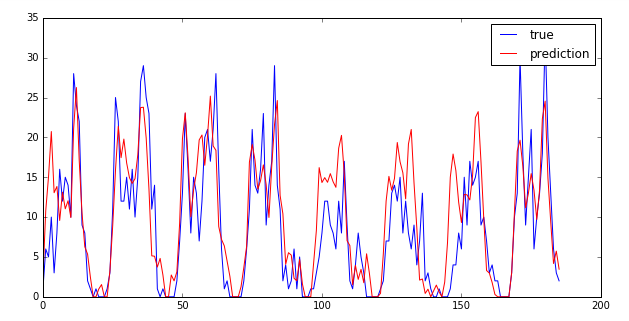
\includegraphics[width=\columnwidth]{station_229ar.png}
	\caption{At the Great Jones St stationthe daily trends were consistent and easy to model}
	\end{center}
\end{figure}
\begin{figure}[!hbt]
	\begin{center}
	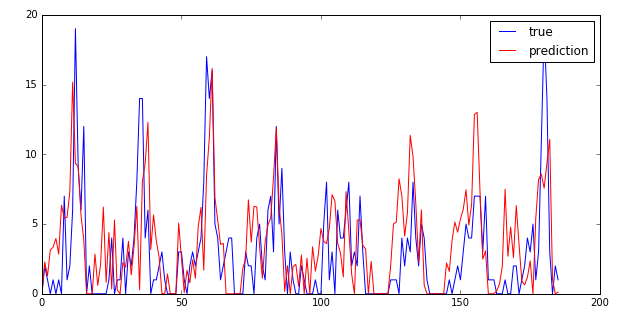
\includegraphics[width=\columnwidth]{station_150ar.png}
	\caption{At the E 2 St \& Avenue C station the trends were less consistent and not as easy to model}
	\end{center}
\end{figure}





\subsection{Neighborhood-based}



\begin{figure}[!hbt]
	\begin{center}
	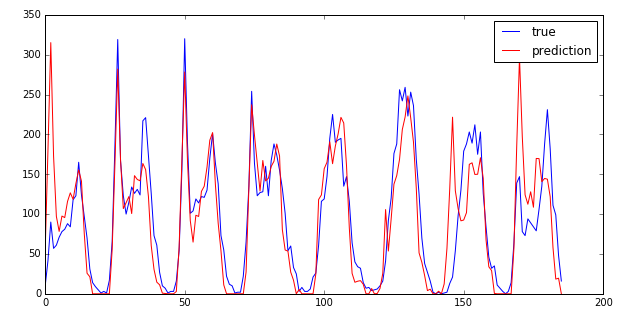
\includegraphics[width=\columnwidth]{cluster_24ar.png}
	\caption{Modeling at a high use cluster}
	\end{center}
\end{figure}
\begin{figure}[!hbt]
	\begin{center}
	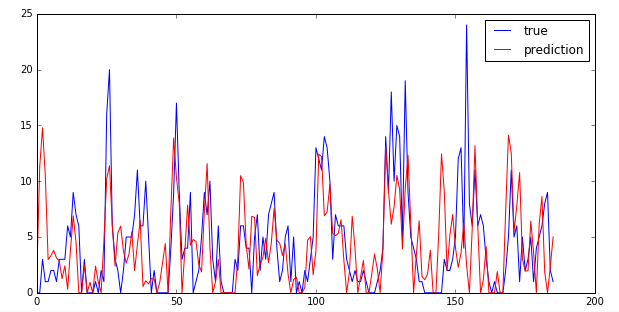
\includegraphics[width=\columnwidth]{cluster_11ar.png}
	\caption{Lower traffic clusters were not as easy to model}
	\end{center}
\end{figure}


\subsection{Bike Angels Program}


\section{Live Predictions on the Web}
A live dashboard showing both the AR predictions we make and current system status is available to view at http://live.status.bike/. We include views for both Neighborhood level predictions and status as well as station-level. The predictions update every hour, and the current status updates as quickly as Citi Bike updates their live status. The web server was built using the Flask framework in Python. We forgo a SQL layer in favor of the Python Pandas for a lightweight way to merge the different data sources and format the output JSON in an easy-to-digest manner for the front end. The main function of the Flask app is to build API's for both the cluster and station-level predictions. The output of the /clusters api is GeoJSON, which integrates easily into the front end. The output of the /stations api is regular JSON. Both APIs give statuses and predictions for the entities they describe, and are cached every 50 seconds to improve performance and scalability. The Flask app also returns the HTML template for the map, but all of the HTML rendering is done on the client. The front end was built using React in ES6 and transpiled to browser-readable Javascript using Babel and Webpack. The whole web-stack (Node + Python) is created by a Docker image and is hosted on AWS, so deployment is very simple.

\section{Impact}
Live predictions can help with both Citi Bike and their restocking, as well as system users for trip planning.


\section{Additional Resources}

\begin{itemize}
  \item Some computational time to run our optimizer algorithm to generate some query plans.
  \item Access to a machine where we can install and run experiments using our current database prototype.
  \item We will need to use some cloud computing infrastructure to complete this project. In addition we will need to have Spark Streaming working.
 \end{itemize}
 
\section{Related Literature}


\begin{itemize}
\item \emph{Background for the project:} Chen et al. introduce a Dynamic Cluster-based approach to predicting over-demand stations \cite{chen}.  Li. et al. introduce a Gradient Boosting Regression tree model to predict the rate of demand going to and from an individual station.  Zhang et al. introduce a regression model for individual trip destination and length predictions~ \cite{zhang},. We plan on implementing these methods to find which are best at predicting demand in the system.





\item \emph{Work the project relies and builds on: } Some preliminary work has suggested a language for specifying query plans~that we could borrow from.  Also, Recent work~nt ways to store and index data lend credence to the need for different cost models for access data in relations.



Parikh et al. introduce a Markov Model to predict optimal restocking levels of a system \cite{parikh}. Freund et al. consider the problem of optimal dock capacity \cite{freund}.Raviv et al. also have an approach to determinig optimal inventory methods. We will use these approaches to evaluate how CitiBike restocks it's system.

Schuijbroek et al. investigate optimal routing for system rebalancing in bike shares \cite{schu}. We plan on using their approach to evaluate the Citi Angels program.
\end{itemize}


\section{Define Success}


This project will be a success if we can accurately predict systems shortages ahead of time. After the models are fit, we will use them to predict real-time data. With better demand prediction we will be able to evaluate current resource allocation methods. If our model is able to correctly predict outages ahead of time, it will be a success.  Finally, our web visualization will be useful for riders who expect to use the system, and the system operators to make strategic decisions by moving bikes and docks or offering incentives to riders
.

\begin{thebibliography}{2}
\bibitem{zhang}  Zhang, J., Pan, X., Li, M., \& Yu, P. S. (2016). Bicycle-Sharing System Analysis and Trip Prediction. 2016 17th IEEE International Conference on Mobile Data Management (MDM). doi:10.1109/mdm.2016.35
\bibitem{chen}Chen, L., Jakubowicz, J., Zhang, D., Wang, L., Yang, D., Ma, X., . . . Nguyen, T. (2016). Dynamic cluster-based over-demand prediction in bike sharing systems. Proceedings of the 2016 ACM International Joint Conference on Pervasive and Ubiquitous Computing - UbiComp '16. doi:10.1145/2971648.2971652
\bibitem{li} Li, Y., Zheng, Y., Zhang, H., \& Chen, L. (2015). Traffic Prediction in a Bike-Sharing System. Proceedings of the 23rd ACM International Conference on Advances in Geographical Information Systems.

\bibitem{freund} Freund, D., Henderson, S. G., \& Shmoys, D. B. (2016). Minimizing Multimodular Functions and Allocating Capacity in Bike-Sharing Systems. arXiv preprint arXiv:1611.09304.

\bibitem{schu}Schuijbroek, J., Hampshire, R., \& van Hoeve, W. J. (2013). Inventory rebalancing and vehicle routing in bike sharing systems.
Chicago	

\bibitem{parikh} Parikh, P., \& Ukkusuri, S. V. (2014, August). Estimation of Optimal Inventory Levels at Stations of a Bicycle Sharing System. In Transportation Research Board 94th Annual Meeting (No. 15-5170).

\bibitem{raviv} Raviv, T., \& Kolka, O. (2013). Optimal inventory management of a bike-sharing station. IIE Transactions, 45(10), 1077-1093.


\end{thebibliography}

\bibliography{prospectus}
\end{document}